%Simulation Results and Discussion


\subsection{Length of shortest tour}

In a first attempt the dependency of the shortest tour length on different parameters is analysed. Thereby the number of completed rounds each agent finishes is varied. Moreover the relative weighting of deposited pheromone and closeness is analysed by changing the parameter \beta and the value of the update rate \alpha is optimized. \\
The shortest tour length is calculated for a 51 cities problem and averaged over 10 trials. In Figure \ref{fig:roundsp} its dependency on the number of completed tours is shown. As expected the average length decreases asymptotically towards the value of the optimal path. This value is then compared to the known solution from \cite{web:data}. This is also done with the trajectory vector of the shortest tour, i.e. the sequence of city numbers which yields the optimal tour.

\begin{figure}[h!]
\begin{center}
\includegraphics[width=11cm, height= 6 cm]{rounds_vs_shortestpath}
\caption{Shortest tour length averaged over 10 runs for different numbers of rounds. The value approximates the optimal solution for \approx 1200 rounds?}
\label{fig:roundsp}
\end{center}
\end{figure}

Figure \ref{fig:alphasp} illustrates that the averaged shortest path length is optimized for \alpha between 0.1 and 0.3. This is the region where the length of the tour and also the error of the shortest path is minimized. This is why for the following simulations the parameter \alpha is chosen to be 0.1. The reason why the shortest path is highest close to zero and one can be understood considering the pheromone update formulae (\ref{eq:localtauupdate}) and (\ref{eq:globalupdate}) on page \pageref{sec:model}. For $\alpha=0$ the local and global pheromone concentration stays constant, no update is made. Hence the cities are only favored by closeness and not the pheromone concentration anymore. On the other hand, while \alpha 
\begin{figure}[h!]
\begin{center}
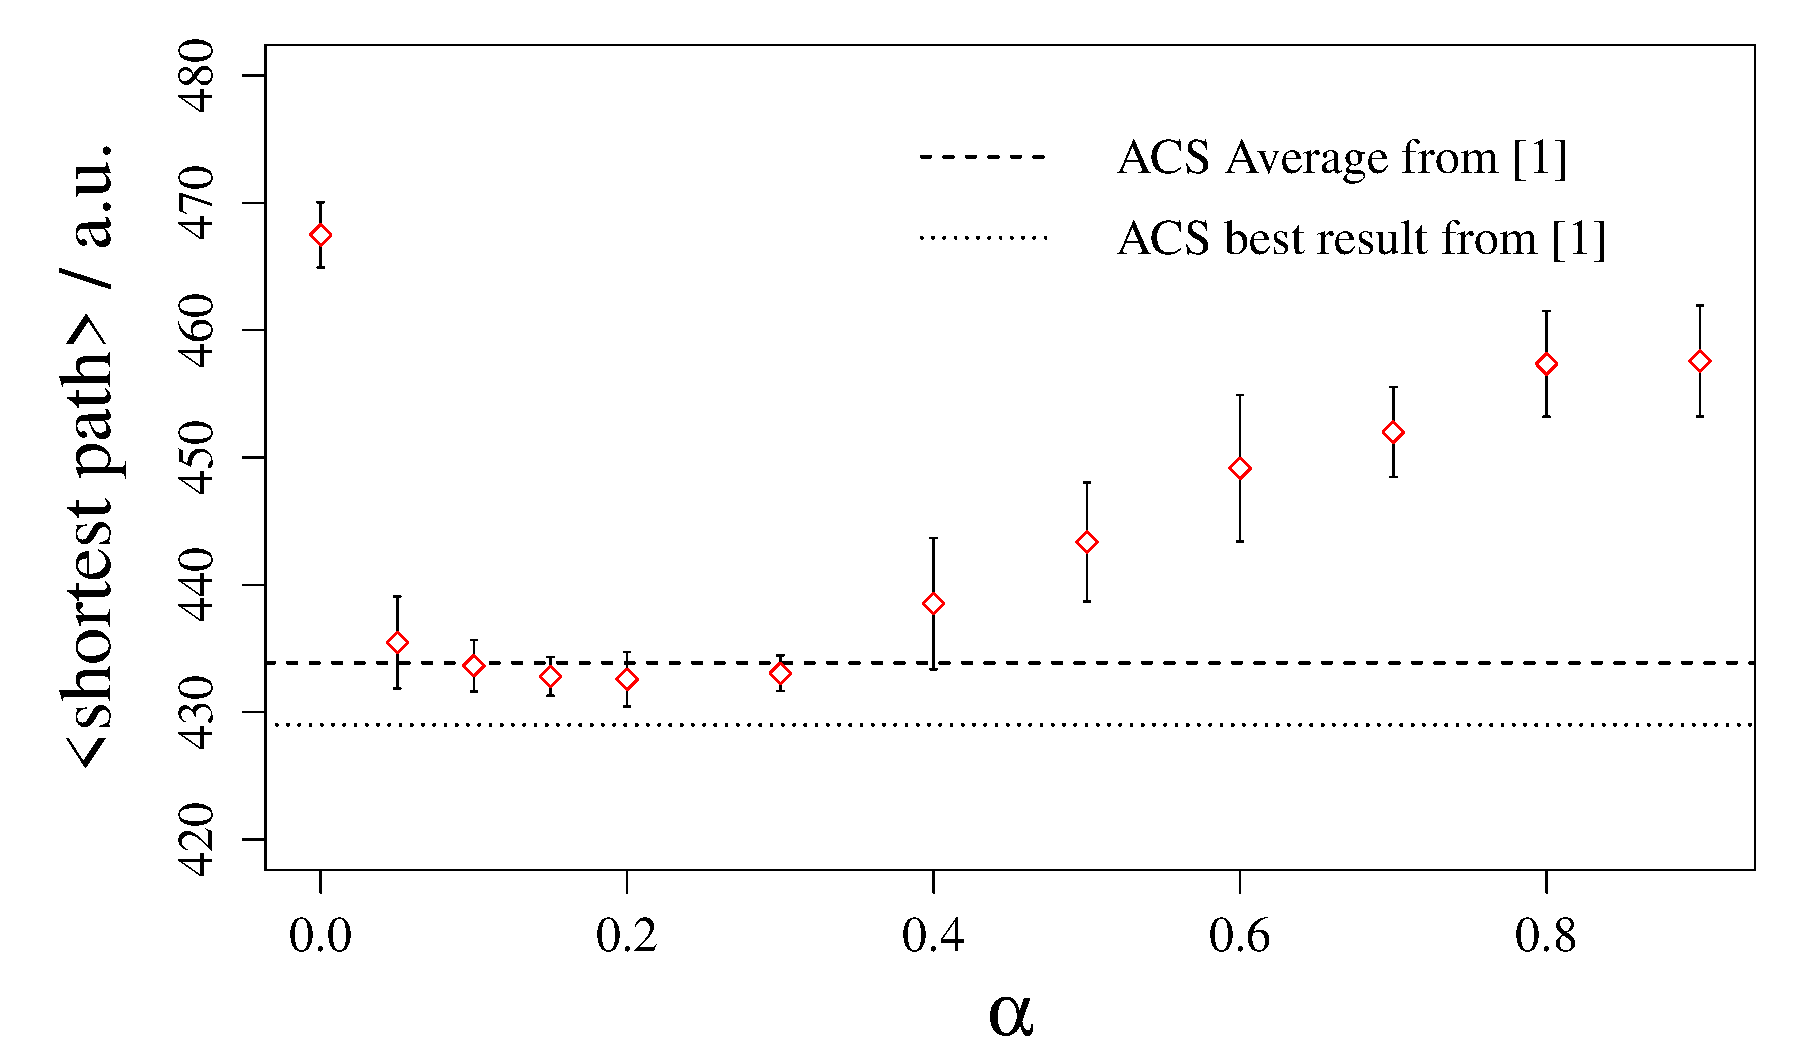
\includegraphics[width=11cm, height= 6 cm]{alpha_vs_shortestpath}
\caption{.}
\label{fig:alphasp}
\end{center}
\end{figure}

\subsection{Model adaptions}

